\usetikzlibrary{calc}
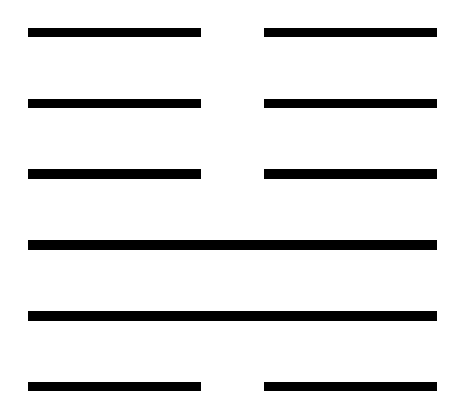
\begin{tikzpicture}[x=1cm,y=1cm,line width=.6pt,font=\normalsize]
  % Chonggua illustration, top-to-bottom: yin, yin, yin, yang, yang, yin.
  % Full length 5.2cm; yin segments 0--2.2 and 3.0--5.2 (gap 0.8cm centered).
  % Bar half-height 0.06cm; row pitch 0.9cm.
  % Top yin (y=4.5)
  \fill[black] (0,4.44) rectangle (2.2,4.56);
  \fill[black] (3.0,4.44) rectangle (5.2,4.56);
  % Second yin (y=3.6)
  \fill[black] (0,3.54) rectangle (2.2,3.66);
  \fill[black] (3.0,3.54) rectangle (5.2,3.66);
  % Third yin (y=2.7)
  \fill[black] (0,2.64) rectangle (2.2,2.76);
  \fill[black] (3.0,2.64) rectangle (5.2,2.76);
  % Fourth yang (y=1.8)
  \fill[black] (0,1.74) rectangle (5.2,1.86);
  % Fifth yang (y=0.9)
  \fill[black] (0,0.84) rectangle (5.2,0.96);
  % Bottom yin (y=0.0)
  \fill[black] (0,-0.06) rectangle (2.2,0.06);
  \fill[black] (3.0,-0.06) rectangle (5.2,0.06);
\end{tikzpicture}
